% ------------------------------------------------------------------
\documentclass[12 pt]{article} % A4 paper set by geometry package below
\pagenumbering{arabic}
\setlength{\parindent}{10 mm}
\setlength{\parskip}{12 pt}

% Nimbus Sans font should be reasonably legible
\usepackage{helvet}
\renewcommand{\familydefault}{\sfdefault}
\usepackage[T1]{fontenc}  % Without this \textsterling produces $

% Section header spacing
\usepackage{titlesec}
\titlespacing\section{0pt}{12pt plus 4pt minus 2pt}{0pt plus 2pt minus 2pt}
\titlespacing\subsection{0pt}{12pt plus 4pt minus 2pt}{0pt plus 2pt minus 2pt}
\titlespacing\subsubsection{0pt}{12pt plus 4pt minus 2pt}{0pt plus 2pt minus 2pt}

\usepackage{amsmath}
\usepackage{amssymb}
\usepackage{graphicx}
\usepackage{verbatim}    % For comment
\usepackage[paper=a4paper, marginparwidth=0 cm, marginparsep=0 cm, top=2.5 cm, bottom=2.5 cm, left=2.5 cm, right=2.5 cm, includemp]{geometry} % TODO: Slightly adjusted to help the \items look better...
\usepackage[pdftex, pdfstartview={FitH}, pdfnewwindow=true, colorlinks=true, citecolor=blue, filecolor=blue, linkcolor=blue, urlcolor=blue, pdfpagemode=UseNone]{hyperref}

% Put module code and last-modified date in footer
\usepackage{fancyhdr}
\pagestyle{fancy}
\fancyhf{}
\renewcommand{\headrulewidth}{0pt}
\cfoot{{\small \thisunit}\hfill \thepage\hfill {\small \moddate}}

% Hopefully address Canvas complaints about pdf tagging
%\usepackage[tagged]{accessibility}
\hypersetup {
  pdfauthor={David Schaich},
  pdftitle={Statistical Physics Tutorial Activity},
}
% ------------------------------------------------------------------



% ------------------------------------------------------------------
\begin{document}
\newcommand{\thisunit}{MATH327 Tutorial (Cycle)}
\newcommand{\moddate}{Last modified 14 Mar.~2024}
\begin{center}
  {\Large \textbf{MATH327: Statistical Physics, Spring 2024}} \\[12 pt]
  {\Large \textbf{Tutorial activity \ --- \ Otto cycle}} \\[24 pt]
\end{center}

This activity will be introduced in our 14 March tutorial, and you'll have the week until our next tutorial on 21 March to work on it.
In particular, in the next lecture we'll define the \textbf{efficiency} of a thermodynamic engine as the amount of work it performs divided by the amount of input heat it needs.
Knowing this, you can start working on this activity by considering the work and heat corresponding to each of the four processes forming the `Otto cycle' shown below, which describes an idealized petrol engine: \\[-24 pt]
\begin{itemize}
  \item Fast (adiabatic) compression increases the pressure of the gas (a mixture of air and vaporized petrol), until a spark ignites it.
  \item This ignition introduces lots of heat almost instantaneously, while the volume is fixed at $V_2$.
        Even though the gas itself is burning, we can interpret this heat as coming from energy exchange with a hot thermal reservoir.
  \item The gas then does work by adiabatically expanding back to volume $V_1 > V_2$.
  \item Finally, heat is expelled at fixed volume $V_1$ by swapping the hot exhaust for an equal amount of cooler, fresh gas ready to be burned.
\end{itemize}

\begin{center}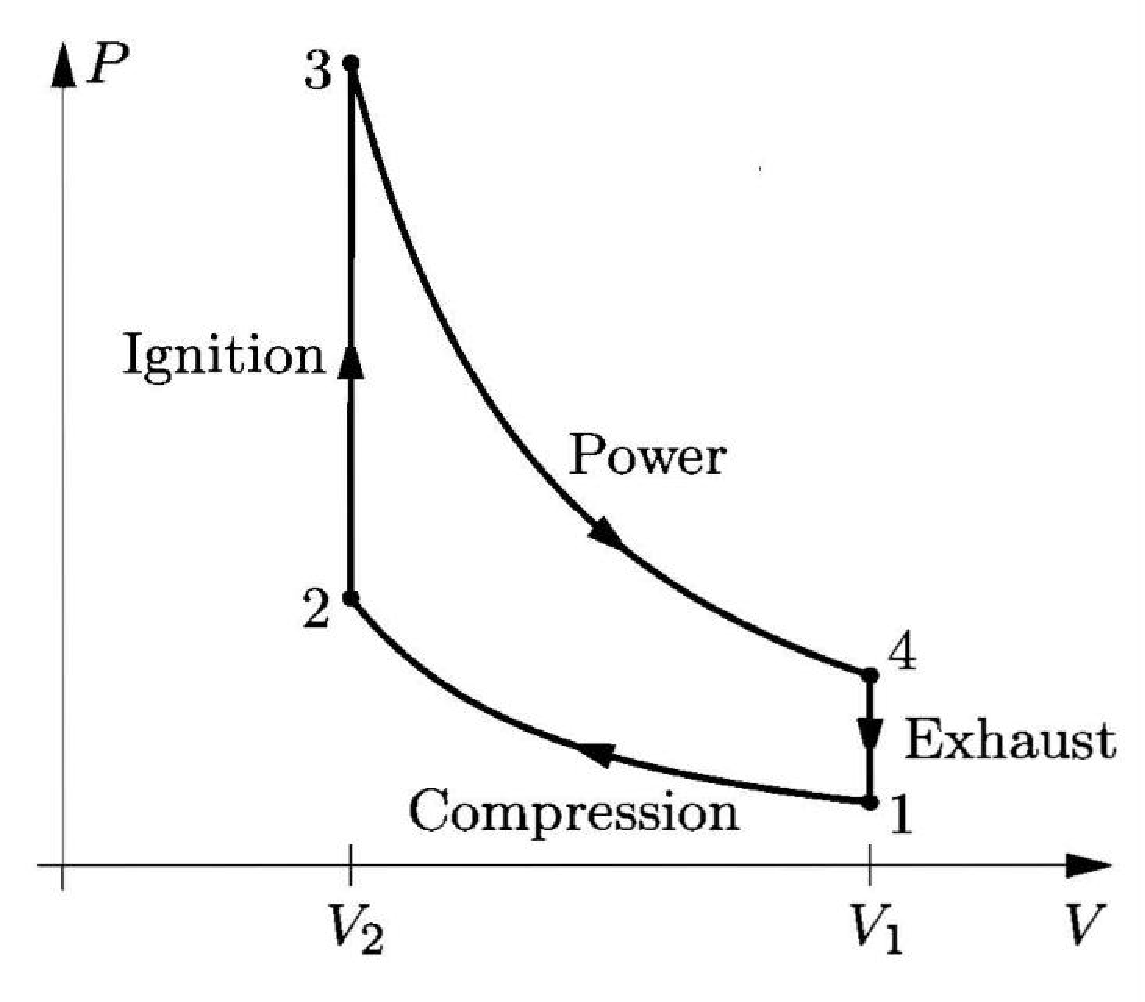
\includegraphics[width=0.6\textwidth]{figs/Otto.pdf}\end{center}

The efficiency $\eta$ of the Otto cycle depends on the \textbf{compression ratio}
\begin{equation*}
  r \equiv \frac{V_1}{V_2} > 1.
\end{equation*}
What is this efficiency?
How does it compare to the efficiency of the Carnot cycle?
How should $V_1$ and $V_2$ be chosen to maximize the efficiency?

\textbf{Hint:} Given the labels in the PV~diagram above, $T_1$ is the low temperature of the cold reservoir while $T_3$ is the high temperature of the hot reservoir.
The corresponding Carnot cycle efficiency is therefore $\eta_C = 1 - \frac{T_1}{T_3}$, and the comparison is easiest if the Otto cycle efficiency is expressed in terms of temperatures rather than volumes.

\end{document}
% ------------------------------------------------------------------
